%\documentclass[handout]{beamer}
\documentclass{beamer}
\usetheme{Madrid}
\usepackage{comment}
\usepackage{ragged2e}
\usepackage{amsmath}
\usepackage{xcolor}
\usepackage{multirow}
\usepackage{multicol}
\usepackage{caption}
\usepackage{tikz}
\usetikzlibrary{shapes.multipart}
\usetikzlibrary{calc}
\usepackage{booktabs}
\usepackage{tabu}
\usetikzlibrary{arrows}
\usepackage[title]{appendix}
\usepackage{booktabs}
\usepackage{appendixnumberbeamer}
\setbeamertemplate{caption}[numbered]
\usepackage{hyperref}
\hypersetup{
	colorlinks=false,
	linkcolor=blue,
	filecolor=blue,      
	urlcolor=blue,
}

\usepackage{natbib}

\def\boxit#1{%
	\smash{\color{red}\fboxrule=1pt\relax\fboxsep=2pt\relax%
		\llap{\rlap{\fbox{\vphantom{0}\makebox[#1]{}}}~}}\ignorespaces
}
\renewcommand{\today}{\ifcase \month \or January\or February\or March\or %
	April\or May \or June\or July\or August\or September\or October\or November\or %
	December\fi, \number \year} 






\tikzstyle{startstop} = [rectangle, rounded corners, minimum width=2cm, minimum height=0.75cm,text centered, draw=black, fill=red!30]

\tikzstyle{startstop1} = [rectangle, rounded corners, minimum width=2cm, minimum height=0.75cm,text centered, draw=black, fill=blue!30]

\tikzstyle{startstop2} = [rectangle, rounded corners, minimum width=2cm, minimum height=0.75cm,text centered, draw=black, fill=yellow!30]

\tikzstyle{startstop20} = [rectangle, rounded corners, minimum width=1cm, minimum height=0.5cm,text centered, draw=black, fill=yellow!30]

\tikzstyle{startstop3} = [rectangle , rounded corners, minimum width=0.5cm, minimum height=0.75cm,text centered,draw=black]


\tikzstyle{io} = [trapezium, trapezium left angle=70, trapezium right angle=110, minimum width=2cm, minimum height=0.75cm, text centered, draw=black, fill=blue!30]



\tikzstyle{process} = [rectangle, minimum width=2cm, minimum height=1cm, text centered, draw=black, fill=green!30]

\tikzstyle{decision} = [diamond, minimum width=0.75cm, minimum height=0.75cm, text centered, draw=black, fill=green!30]

\tikzstyle{arrow} = [thick,->,>=stealth]




\title[Connected Stocks  via Business Groups]{Connected Stocks via Business Groups:}
\subtitle{Evidence from an Emerging Market}
%\subtitle{}
\author[Aghajanzadeh, Heidari \& Mohseni]{S.M. Aghajanzadeh \qquad M. Heidari \qquad M. Mohseni }
\institute[TeIAS]{Tehran Institute for Advanced Studies }


\begin{document}
	\maketitle
	
	
	
	\section{Motivation}
	
		\begin{frame}{Co-movement and common ownership}
				\begin{figure}
						\centering  
						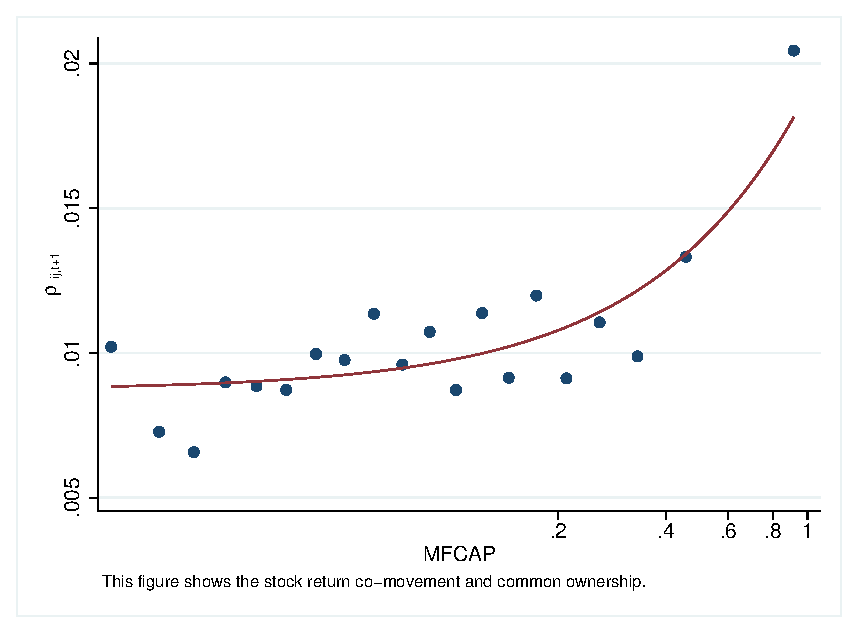
\includegraphics[width=0.85\linewidth]{"Output/mcorr50.eps"}
					\end{figure}
			\end{frame}   
		
			\begin{frame}{Co-movement and common ownership}
					\begin{figure}
							\centering  
							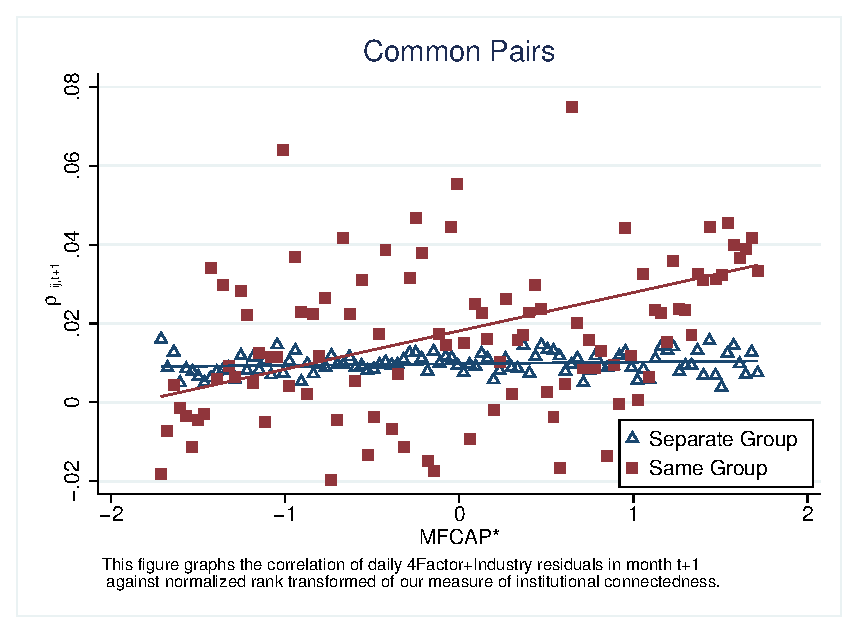
\includegraphics[width=0.85\linewidth]{"Output/mcorr5bg.eps"}
						\end{figure}
				\end{frame}   
	

	\section{Literature}
	
	
	
	
	
	
	
	
	\normalsize
	

	
	
	\subsection{Related Literature}
	\begin{frame}{Related Literature}\label{Grapgh}
		\resizebox{\textwidth}{!}{
			\tikzstyle{startstop1} = [rectangle, rounded corners, minimum width=2cm, minimum height=0.75cm,text centered, draw=black, fill=blue!30]
	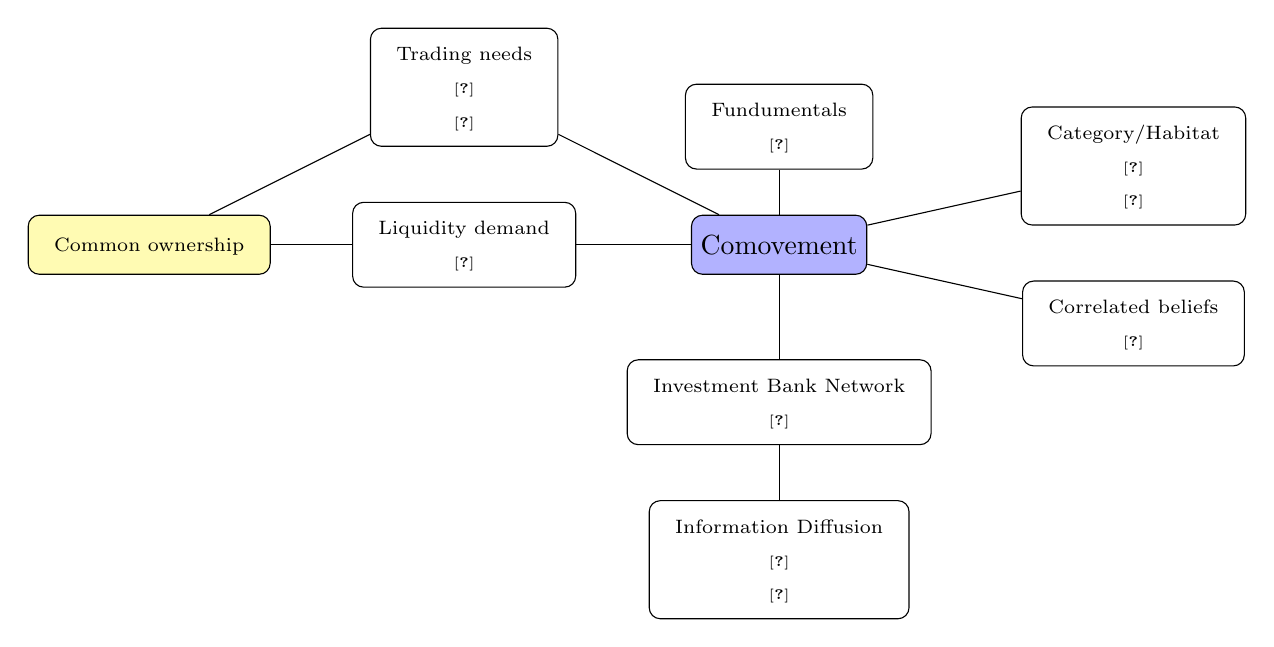
\begin{tikzpicture}[node distance=1cm][every text node part/.style={align=center}]
		
		
		
		\node (comovement) [startstop1] {Comovement};
		
		\pause
		
				\node (Fundumental) [startstop3,above of = comovement , yshift=0.5cm , xshift=0cm ] { \begin{tabular}{c}
				\scriptsize	Fundumentals	\\ \tiny\cite{shiller1989comovements}
		\end{tabular} };
		
		
		\draw (Fundumental) -> (comovement);
		
		
		\pause
		
		\node (categoryhabitat) [startstop3,above of = comovement , yshift=0cm , xshift=4.5cm ] { \begin{tabular}{c}
				\scriptsize	Category/Habitat	\\ \tiny\cite{barberis2005comovement}\\ \tiny\cite{barberis2003style}
		\end{tabular} };
		
		
		\draw (categoryhabitat) -> (comovement);
		
		\pause
		\node (belief) [startstop3,below of = comovement , yshift=0cm , xshift=4.5cm ] {\begin{tabular}{c}\scriptsize
				Correlated beliefs	\\
				\tiny\cite{david2016correlated}
		\end{tabular}};
		
		\draw (belief) -> (comovement);
		
		\pause
		
		\node (investmentbanking) [startstop3,below of = comovement , yshift=-1cm , xshift=0cm ] {\begin{tabular}{c}\scriptsize
				Investment Bank Network \\
				\tiny\cite{grullon2014comovement}
		\end{tabular}};
		
		\draw (investmentbanking) -> (comovement);
		
		
		
		\pause
		\node (information) [startstop3,below of = investmentbanking , yshift=-1cm , xshift=0cm ] {\begin{tabular}{c}\scriptsize
				Information Diffusion	\\\tiny\cite{pantzalis2017shareholder}\\
				\tiny\cite{HAMEED2019103}
		\end{tabular}};
		
		\draw (information) -> (investmentbanking);
		
		\pause
		
		
		
		
		
		
		
		%% common ownership
		\node (commonownership) [startstop2,left of = comovement , yshift=0cm , xshift=-7cm ] {\begin{tabular}{c}\scriptsize Common ownership  \end{tabular}};
		\pause
		\node (trading) [startstop3,right of = comovement , yshift=2cm , xshift=-5cm ] { \begin{tabular}{c}
				\scriptsize	Trading needs\\ \tiny \cite{greenwood2011stock} \\  \tiny \cite{AntonPolk}
		\end{tabular} };
		
		\draw (commonownership) -> (trading);
		\draw (trading) -> (comovement);
		\pause
		\node (liquidity) [startstop3,below of = trading , yshift=-1cm , xshift=0cm] {\begin{tabular}{c} \scriptsize Liquidity demand \\ \tiny \cite{Liquidity2016}  \end{tabular}};
		
		\draw (commonownership) -> (liquidity);
		\draw (liquidity) -> (comovement);
		

		
		
%		\node (corporate) [startstop3,below of = liquidity , yshift=-1cm , xshift=0cm ] {  \begin{tabular}{c}
%				\scriptsize	Poor corporate governance	\\ \tiny \cite{khanna2009synchronicity}
%		\end{tabular}};
%		
%		\draw (commonownership) -> (corporate);
%		\draw (corporate) -> (comovement);
	\end{tikzpicture}

		}
		
		%		\hfill
		%		\hyperlink{maineffect}{\beamerbutton{Papers}}
	\end{frame}
	
	\begin{frame}{Model Estimation}{Normalized Rank-Transformed}
	\label{mresult2part1} 
	\begin{table}[htbp]
		\centering
		\resizebox{0.8\textwidth}{!}{
			{
\def\sym#1{\ifmmode^{#1}\else\(^{#1}\)\fi}
\begin{tabular}{l*{6}{c}}
\hline\hline
                    &\multicolumn{6}{c}{Dependent Variable:  Future Pairs's Comovement}                                                                 \\\cmidrule(lr){2-7}
                    &\multicolumn{1}{c}{(1)}         &\multicolumn{1}{c}{(2)}         &\multicolumn{1}{c}{(3)}         &\multicolumn{1}{c}{(4)}         &\multicolumn{1}{c}{(5)}         &\multicolumn{1}{c}{(6)}         \\
\hline
$ \text{MFCAP*} $   &     0.00600\sym{***}&     0.00328\sym{***}&                     &                     &     0.00104         &    0.000929         \\
                    &      (8.10)         &      (4.87)         &                     &                     &      (1.68)         &      (1.53)         \\
[1em]
SameGroup           &                     &                     &      0.0358\sym{***}&      0.0254\sym{***}&      0.0242\sym{***}&      0.0219\sym{***}\\
                    &                     &                     &      (9.99)         &      (8.45)         &      (8.21)         &      (7.02)         \\
[1em]
SameIndustry        &                     &      0.0267\sym{***}&                     &      0.0216\sym{***}&      0.0212\sym{***}&      0.0215\sym{***}\\
                    &                     &      (7.39)         &                     &      (6.81)         &      (6.72)         &      (6.80)         \\
[1em]
SameBM              &                     &      0.0224\sym{***}&                     &      0.0213\sym{***}&      0.0214\sym{***}&      0.0199\sym{***}\\
                    &                     &      (6.41)         &                     &      (6.09)         &      (6.16)         &      (5.77)         \\
[1em]
SameSize            &                     &      0.0123\sym{**} &                     &      0.0143\sym{***}&      0.0138\sym{***}&      0.0254\sym{***}\\
                    &                     &      (3.24)         &                     &      (3.85)         &      (3.71)         &      (5.56)         \\
[1em]
CrossOwnership      &                     &      0.0600\sym{***}&                     &      0.0300\sym{*}  &      0.0316\sym{*}  &      0.0377\sym{**} \\
                    &                     &      (5.50)         &                     &      (2.36)         &      (2.48)         &      (2.93)         \\
[1em]
Constant            &      0.0142\sym{***}&      0.0204\sym{***}&      0.0103\sym{***}&      0.0187\sym{***}&      0.0188\sym{***}&      0.0280\sym{***}\\
                    &     (12.80)         &      (8.91)         &      (9.42)         &      (7.99)         &      (8.04)         &      (9.43)         \\
\hline
PairType Control    &          No         &          No         &          No         &          No         &          No         &         Yes         \\
Observations        &      389591         &      389591         &      389591         &      389591         &      389591         &      389591         \\
\hline\hline  \end{tabular}}

		}
	\end{table}
	
	
\end{frame}
\begin{frame}{Model Estimation}{Normalized Rank-Transformed}
	\label{mresult2part2} 
	\begin{table}[htbp]
		\centering
		\resizebox{1\textwidth}{!}{
			{
\def\sym#1{\ifmmode^{#1}\else\(^{#1}\)\fi}
\begin{tabular}{l*{4}{c}}
\hline\hline
                &\multicolumn{4}{c}{Dependent Variable:  Future Pairs's Comovement}         \\\cmidrule(lr){2-5}
                &\multicolumn{1}{c}{(1)}         &\multicolumn{1}{c}{(2)}         &\multicolumn{1}{c}{(3)}         &\multicolumn{1}{c}{(4)}         \\
\hline
$ \text{MFCAP*} $&  0.00920\sym{***}&-0.0000508         &-0.000111         & 0.000283         \\
                &   (7.05)         &  (-0.08)         &  (-0.18)         &   (0.60)         \\
[1em]
SameGroup       &                  &                  &  0.00925\sym{**} &  0.00684         \\
                &                  &                  &   (2.73)         &   (1.82)         \\
[1em]
 $ \text{MFCAP}^* \times {\text{SameGroup} }  $ &                  &                  &   0.0123\sym{***}&   0.0119\sym{***}\\
                &                  &                  &  (10.11)         &   (9.41)         \\
\hline
Sub-sample      &SameGroup         &   Others         &      All         &      All         \\
Business Group FE&       No         &       No         &       No         &      Yes         \\
Observations    &    47941         &   350877         &   398818         &   398818         \\
\hline\hline
\multicolumn{5}{l}{\footnotesize \textit{t} statistics in parentheses}\\
\multicolumn{5}{l}{\footnotesize \sym{*} \(p<0.05\), \sym{**} \(p<0.01\), \sym{***} \(p<0.001\)}\\
\end{tabular}
}

		}
	\end{table}
\end{frame}
	
	\normalsize
	
		\appendix
	
	\tiny
\begin{frame}[allowframebreaks]{References}
	
	{		
		\bibliographystyle{apalike}
		\bibliography{Ref}
	}
\end{frame}
	
\end{document}